\label{ch:methods}

\section{Methods}

\subsection{Data Collection}

The Jena Experiment:

\begin{itemize}
\item N\ang{50;55;} E\ang{11;35;} ; 130 m a.s.l.
\item	Established in 2002
\item	Total Size: 10 hectars
\item	Arable field for 40 years before experiment started (therefore strongly fertilized)
\item	Plots are mowed every June and September
\item	Main experiment has 82 plots, each 20x20m (400m$^2$ )
\item	Originally sown species mix of 1,2,4,8,16 or 60 species, divided into four blocks (randomized complete block design) along abiotic gradients (mainly soil sand content)
\item	Part of the Plot is weeded twice a year (not my sampling area)
\end{itemize}


\subsubsection{Choosing Species and Plots}

The parts of the plots with continuous weeding were normally very scarce with flowers and had a very low species richness. So I collected the data in the “old invasion plots” (4m x 5.5m , 22m$^2$ ) and in the “new invasion plots” (5m x 3.5m, 17.5m$^2$ ) with a much higher cover, species richness and diversity. The "old invasion plots" were not weeded since the first seeding in 2002. The "new invasion plots" were not weeded since 2009.\\

I chose 5 species to observe (Those species were chosen because they were present in min. 5 plots with a differing frequency):


\begin{table}[htbp]
  \centering
  \caption{Focal Species}
    \begin{tabular}{llllll}
    \toprule
    \textbf{Short} & \textbf{Name} & \textbf{German Name} & \textbf{Order} & \textbf{Family} & \textbf{Color} \\
    \midrule
    Ono   & Onobrychis viciifolia & Saat-Esparsette & Fabales & Fabaceae & pink+white \\
    Lat   & Lathyrus pratensis & Wiesen-Platterbse & Fabales & Fabaceae & Yellow \\
    Lot   & Lotus corniculatus & Gewöhnliche Hornklee & Fabales & Fabaceae & Yellow \\
    Ger   & Geranium pratense & Wiesen-Storchschnabel & Geraniales & Geraniaceae & Purple \\
    TP    & Trifolium pratense & Wiesen-Klee & Fabales & Fabaceae & Purple \\
    \bottomrule
    \end{tabular}%
  %\label{tab:addlabel}%
\end{table}%


Because the vegetation changed very quickly (heavy rain and very warm temperatures alternating) I chose max. 7 plots (= 14h) to observe at a time. 
Every time I finished a session I did a new sampling of all 82 plots of the Jena Experiment to check for suitable plots with focal plant species and their frequencies for the next round. Those observations were randomly distributed over the next days to prevent time dependencies ( observation times over the whole day for each plot)


\subsubsection{The Sampling}

\begin{itemize}
\item	Observations were made only during good weather conditions (max partly overcast, no rain, max light wind, min. 15 degree)
\item	Sampling time between 9am and 5pm (there was normally heavy fog and moist in the mornings so I could only start sampling from 10 or even 11)
\item	Sampling occurred between 20.7. -  12.8. 
\item Total of 15 sampling days (due to weather conditions)
\end{itemize}



\begin{figure}
\centering
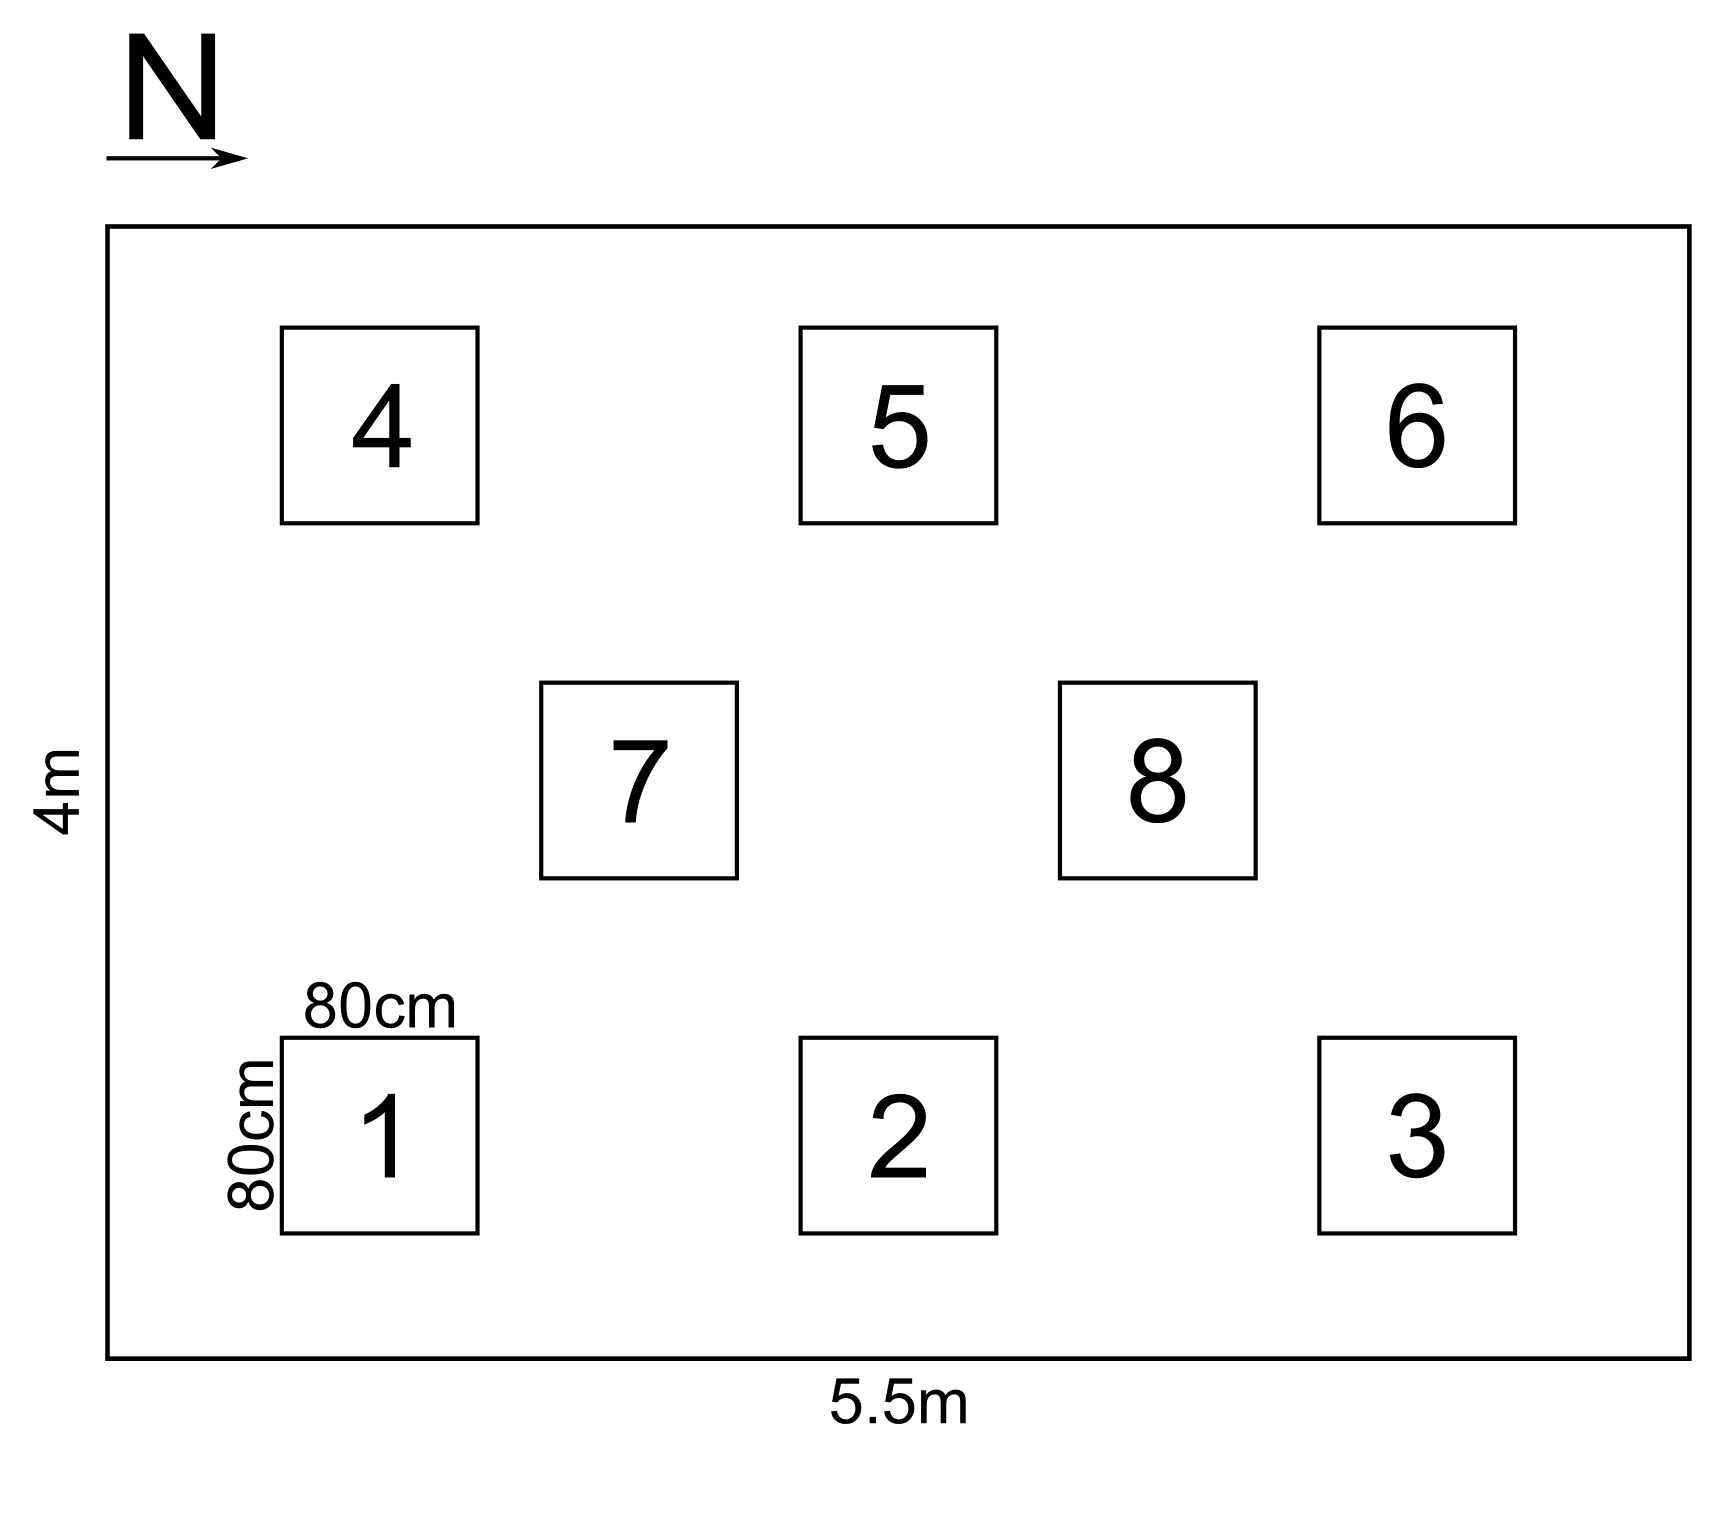
\includegraphics[width=9cm]{Images/plot-design}
 \caption{The sampling design within a plot}
 \label{fig:plot-design}
\end{figure}




\begin{itemize}
\item The pollinators were divided into bees, bumblebees, hoverflies and “other”
\item sampled eight of the 80x80cm patches per plot to get 2h of data per frequency and get a good mean over the plot (flowers were often in clusters and not distributed over the whole plot)
\item Patches were distributed as shown in Figure~\ref{fig:plot-design}
\end{itemize}

\begin{itemize}
\item When the flowers were very unevenly distributed over the Plot (which happened especially at low frequencies) I chose to observe some patches which contained flowers of the chosen species twice
\item I normally observed two species at once to save time/get a larger dataset. If there were not too many flowers that was easy feasible. If there were Plots with unevenly distributed flowers as explained above I observed the regular 1-8 patches for the evenly distributed species and additionally doubling patches for the uneven species. 
\item Eg. Geranium was flowering at all 8 patches, Lotus only in the southern part (patch 1,2,4,5, and 7). I regularly observed all patches 1-8 for Geranium. Because I was missing 3 patches for Lotus I doubled 1, 7 and 5. During this doubling I still kept track of visitors of the Geranium flowers. So in the end my dataset was the following:
\begin{itemize}
	\item 8+3 Geranium observations
	\item 8 Lotus observations
\end{itemize}
\end{itemize}


\subsection{Statistical Analysis}

\subsubsection{The Data}

Within the 4 weeks of sampling I got 386 entries, each equivalent to 15min of observation

\begin{itemize}
\item Flower visits to the focal species within the patch (divided by pollinator type)
\item Flower visits to other flowers except the focal species in the patch (divided by pollinator type)
\item Species Richness in the Patch (with names)
\item Species Richness in the Plot (with names and quantities)
\item Floral Cover in Patch and Plot (own estimation)
\item Frequency of the focal species in Patch and Plot
\item Count of individual flowers respectively inflorescence of the focal species
\item PlotID
\item PatchID
\item Date/Time
\end{itemize}

\subsubsection{The Analysis}


mixed model (lme,lmer,glmer) --> glmPQL für p-values

response variable: Per-Flower visitation rate (summed or by pollinator-subfamily) (poisson)

fixed: frequency, species richness, flower cover

random: specID (bin nicht interessiert an der Pflanze sondern an einer allgemeingültigen Aussage, Blüten waren sehr unterschiedlich in der Attraktivität)

- was ist mit PlotID und PatchID?
- ich habe 8 Observations pro Plot, die eigentich irgendwie zusammen gehören...
- Similarity-gradient statt einfach SR?
- Plot position könnte wichtig sein, näher an beehive oder die Pflanzenzusammensetzung
- Habe auch Daten zur Visitation Rate aller anderen Arten, ralative Vr interessant?


Backwards selection with AIC




\newpage


\subsection{The Model}


\subsubsection{About ABMs}
Agent-Based Model (ABM, also known as Individual-Based Model IBM) are a valuable tool for assessing interactions in an ecosystem. Every agent behaves independently after simple behavior rules. 
Very good for testing behavior change with changing environmental conditions (eg. nectar reward or flower quantity)

NetLogo \citep{wilensky1999netlogo} is a simple programming environment for ABMs and connectable with R through the RNetLogo-Package.

Agent-based models get more attractive throughout the modeling community of various research areas. Foraging models also grew in number over the last years.



\citet{faruq2013biological} compared the foraging success while applying different color wavelengths.

\citet{dornhaus2006benefits} looked at the benefits of a recruitment system and colony sizes.
 
\citet{bukovac2013bees} simulated the difference between the parallel visual scan of honey bees and the serial visual scan of bumble bees to for the ability to avoid distractions during foraging. 

\citet{dyer2014bee} trained honey bees in a lab experiment to fine color discrimination to check for their flexibility to change when the reward changes between flower types. Afterwards,  \citet{dyer2014bee} confirmed the findings with a ABM. 

The ABM of \citet{hanoteaux2013effects} showed reproduction success of plants in a combination of spatial arrangement and relative frequency of flowers with unequal attraction to the pollinator. 



\subsubsection{The Environment}

In NetLogo, the "world" contains a spatial grid with a set number of cells called patches. Agents are not spatially explicit and can move freely over the patches according to their given behavior rules. Patches and agents can both have own properties and can interact with each other. 
In my model, the "meadow" has 100x100grid cells with horizontally and vertically wrapping to avoid edge effects. Every grid cell can either contain a single flower of one of the two species or grass. The flowers of those two species are randomly distributed over the meadow. Every flower contains 1Joule of floral reward in the beginning of each simulation run. The pollinators ("bee-agents") are also randomly distributed over the modeling environment, no hive is assigned. Bee-agents start without a fixed preference for a flower type but just pick the closest one when the simulation starts. 


\subsubsection{Assumptions}

\begin{itemize}
\item	All pollinators are identical
\item All flowers types are equal (also in terms of reward regrowth, handling times and attractiveness to the pollinator)
\item	Pollinators behave under the theory of flower constancy

\begin{itemize}
\item Change when search is unsuccessful
\item Chance when species is not rewarding any more
\end{itemize}

\item	All bees have a memory for recently visited flowers and gained reward
\item	Pollinators follow the “correlated random walk” if no target is assigned
\item	Energetic costs are ignored
\item	The reward is completely emptied by each visit and can be renewed over time
\item	Pollinators do not communicate
\item	Pollinators only use one trait to choose flower (visual)
\item Pollinators do not have a limit of gained rewards
\item	Pollinators are randomly distributed, no hive is assigned  (no central place foragers)

\end{itemize}

Behavior rules and parameter values are based on empirical research


\subsubsection{Behavior rules}

\begin{figure}
\centering
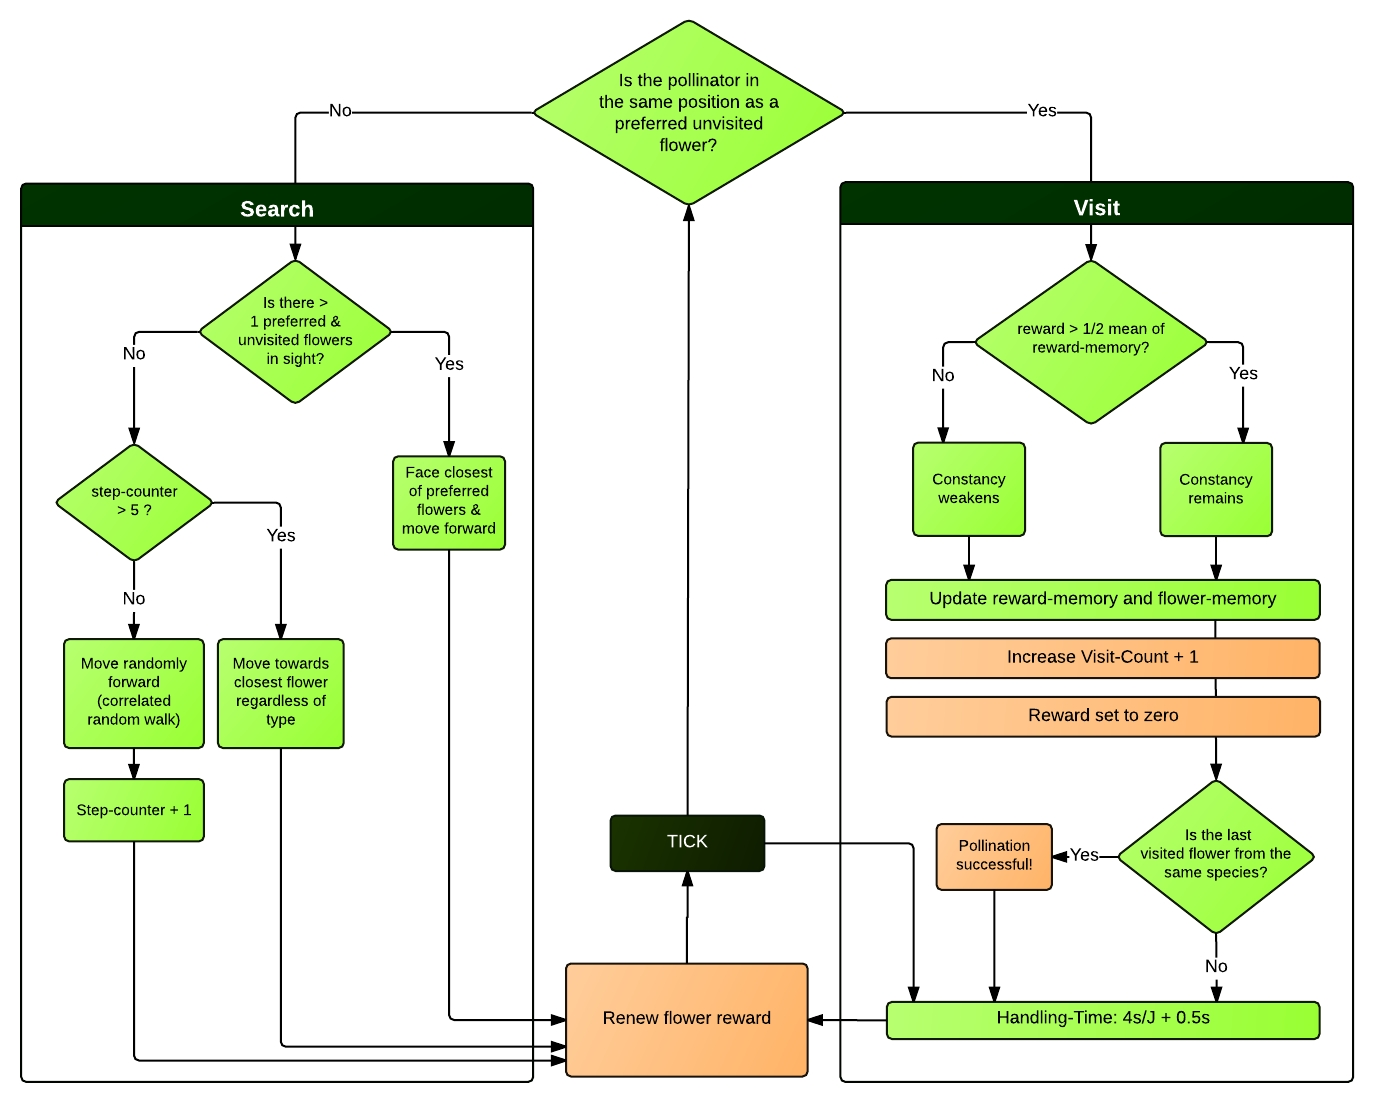
\includegraphics[width=15cm]{Images/flowchart-model}
 \caption{Flowchart describing the behavior rules for the bee-agents within the Agent-Based Model. Every bee-agent can either search for a preferred flower or visit one. While searching, a bee-agent can remember the location of the last four visited flowers to avoid double-encountering. If there is no flower in sight after 5 seconds of CRW it will encounter the next available flower despite its type. When a bee-agent visits a flower it takes all reward within a reward-dependent handling time and compares the amount with its memory. If the reward is low, the agent is more likely to visit the other flower type next time. Successful pollination takes place if the last visited flower was from the same flower type.}
 \label{fig:flowchart}
\end{figure}


All bee-agents act independently from each other after given foraging behavior shown in Figure~\ref{fig:flowchart}. The bee-agent can either search for a flower or visit one. Every tick in NetLogo equals one second. \\

The behavior of the bee-agents is strongly influences by the theory of flower constancy ( e.g.  \citealp{bobisud1975pollinator, chittka1997foraging, thomson1981field, chittka1999flower,  goulson1994model,  goulson1999foraging}). Bee-agents will always be in favor of one of the two flowering species and will not visit the other flower type. This preference can change due to lack of searching success and a series of low rewards of the preferred flower \citep{chittka1997foraging}. Pollinators avoid recently visited flowers \citep{goulson1999foraging}. Every bee-agent is equipped with a memory to remember the location of the last 4 already visited flowers \citep{goulson2000pollinators}.

If there is any preferred and unvisited flower in sight it will turn toward it and move towards the flower. If there is no unvisited, preferred flower in sight the bee agent continues searching. \\

Previous research on the speed of foraging pollinators by \cite{essenberg2012explaining} and \cite{kunin1991few} (see  \citealt{kunin1996pollinator}) gave 0.1m/sec as benchmark. Sequentially, bee-agents can move as fast as 1 grid cell per tick in this model. \\

The vision of pollinators was studied in various experiments using a Y-maze apparatus \citep{dyer2008comparative, wertlen2008detection, ne2001effect}. In this model, every bee-agent can detect flowers from a distance of 0.7m with an equivalent of 6 grid cells. Also, it is reduced to a 180$^{\circ}$ cone-shaped field to the front of the agent.\\

Pollinators tend to keep their direction while foraging \citep{waddington1980flight}. In the model, I used a correlated random walk (CRW) to achieve a relatively natural  movement \citep{bartumeus2005animal, codling2008random,  pyke1992flight, viswanathan2008levy}. \\

Empirical studies have shown a higher probability to abandon the original flower preference the longer the search remains unsuccessful \citep{chittka1997foraging}. Therefore will the bee-agent forage on the next available flower regardless its species after 5 seconds (= 5 ticks) of CRW without finding any preferred and unvisited flower. \\

When a bee-agent encounters a preferred and unvisited flower it takes up all its reward in a reward-dependent handling time. The maximal reward a flower can contain is 1J and refills each tick by a linear function.  A bee-agent requires 4 seconds to extract one Joule of reward plus an additionally reward-independent handling time of 0.5 seconds (\citealt{roubik1992ecology} in  \citealt{kunin1996pollinator}). 

The reward taken is stored in the agent-own reward-memory. Every agent can remember the last four receives rewards. When visiting a flower, the bee-agent compares this memory with the current reward quantity. If the reward is less than half the average in the memory, the likelihood to abandon flower constancy and visit another flower type next increases \citep{chittka1997foraging, keasar1996innate}. 

For simplicity reasons, the pollen carryover rate for successful pollination is just one visit. If the last visited flower was the same species, successful pollination takes place ( \citealt{campbell1986predicting}; \citealt{benadi2012population} but see \citealt{montgomery2009pollen} ).


After full collection of the reward, the bee-agent updates its flower-memory and its reward-memory and continues foraging. Each visit and successful pollination is recorded for later analysis. 


%% ------------------------------------

\begin{sidewaystable}[htbp]
\footnotesize
  \centering
  \caption{Parameter values}
    \begin{tabular}{l l l l l l}
    \toprule
    \textbf{Parameter} & \textbf{Description} & \textbf{NetLogo-Type} & \textbf{Type} & \textbf{Value} & \textbf{Reference} \\
    \midrule
    \addlinespace[0.2cm]
    area  & "world" in NetLogo, number of grid-cells &       & integer & 100x100 &  \\
    
    patch-size & Size one grid-cell in NetLogo. Can be either a flower or grass &       & float & 0.1m² &  \\
    
    tick  & One time-unit in NetLogo &       & integer & 1s    &  \\
    
    number-bees & Initial number of pollinators in the model & global & integer &       & 0.0004 - 1 bee/m² \citep{essenberg2012explaining} \\
    
    flower-cover & Proportion of grid cells containing a flower & global & integer &       &  \\
    frequency & Proportion of flowers which are species A  
feq(B) = 100 - freq(A) & global & integer &       &  \\

search-speed & Distance a pollinator can move per tick & bees-own & integer & 0.1m /sec  & \begin{tabular}{@{}l@{}} \citep{kunin1991few} in \citep{kunin1996pollinator}  \\  0.09-0.17 \citep{essenberg2012explaining} \end{tabular} \\

    stdev-angle & Standard deviation for the normal distribution used in the CRW & global & integer & 65    & \citealt{waddington1980flight}  \\
    
    flightsteps-until-change & seconds of unsuccessful search before the constancy changes & bees-own & integer & 5s ( = 5 ticks) &  \citealt{chittka1997foraging}  \\
    
    length-memory & How many flowers can a bee remember to avoid double-visiting.  & bees-own & integer & 4     & \citealt{goulson2000pollinators}, see \citealt{goulson1999foraging} for review \\
    
    view  & Value for the radius of grid-cells a pollinator can see (cone-view of 180°) & bees-own & integer & 0.7m ( = 6 grid-cells) &  \begin{tabular}{@{}l@{}} \citep{dyer2008comparative, wertlen2008detection} \\ \citealt{ne2001effect} \end{tabular} \\
    
    reward-function & How fast the reward is renew per second & flowers-own & float & 0.00004 J/s   &  \\
    handling-time & The time a pollinator needs for exploiting the floral reward & bees-own & integer & reward * 4s + 0.5s & \citealt{roubik1992ecology} in \citealt{kunin1996pollinator} \\
    
    reward & \begin{tabular}{@{}l@{}}Reward in Joule the flower has to offer. \\  Exploited with each visit, renewed over time \end{tabular} & flowers-own   & float & reward(max) = 1J & \citealt{kunin1991few} in \citealt{kunin1996pollinator}  \\
    
    pollen carry-over rate & The max. number of visits within a successful pollination is possible & flowers-own & integer & 1     &  \\
    
    flower-memory & A list of flower-locations  & bees-own & string &       & see \citealt{goulson1999foraging} for review) \\
    reward-memory & A list of the last rewards & bees-own & string &       &  \\
    change-prob & Probability to change the preferred flower type. Increases with low reward & bees-own & float &       &  \\
    spec-last-visit & The species of the last visited flower (for pollination) & bees-own & boolean &       &  \\
    pollination-count & Counts the number of successful pollination & flowers-own & integer &       &  \\
    choice & Current flower choice for the pollinator (for constancy) & bees-own & boolean &       &  \\
    array & \begin{tabular}{@{}l@{}} Array of all suitable flowers (referred, non-visited)\\ flowers in sight of the pollinator \end{tabular} & bees-own & Array &       &  \\
    species & Determines the species of the flower & flowers-own & boolean &       &  \\
    end   & Number of time steps until the model ends &       & integer &       &  \\
    \bottomrule
    \end{tabular}%
  \label{tab:addlabel}%
\end{sidewaystable}%

% ------------------------------------


  
